% THE ETHICAL RESEARCHER'S GUIDE TO USING AI TOOLS
% Workshop Presentation
% Presenters: Dr. Awara Bakhtiyar Rasool & Davar Adil Yassin
% University: Salahaddin University-Erbil
% ============================================================================

\documentclass[aspectratio=169,10pt]{beamer}

% THEME & PACKAGES
\usetheme{metropolis}
\usepackage{graphicx}
\usepackage{tikz}
\usetikzlibrary{positioning,shapes,arrows,calc,backgrounds,fit,decorations.pathreplacing,mindmap,trees,shadows}
\usepackage{amsmath,amsfonts,amssymb}
\usepackage{booktabs}
\usepackage{colortbl}
\usepackage{tcolorbox}
\usepackage{qrcode}
\usepackage{fontawesome5}
\usepackage{listings}
\usepackage{hyperref}

% PATHS
\graphicspath{{images/}}

% COLORS (Salahaddin University Style)
\definecolor{salahaddinred}{RGB}{145, 25, 25}
\definecolor{salahaddingold}{RGB}{255, 215, 0}
\definecolor{ukhblue}{RGB}{0,51,102}
\definecolor{ukhlight}{RGB}{0,110,180}
\definecolor{forestgreen}{RGB}{34,139,34}
\definecolor{alertred}{RGB}{204,0,0}
\definecolor{promptbg}{RGB}{245,245,245}

% BEAMER CUSTOMIZATION
\setbeamercolor{title}{fg=salahaddinred}
\setbeamercolor{frametitle}{bg=salahaddinred, fg=white}
\setbeamercolor{progress bar}{fg=salahaddingold,bg=gray!20}
\setbeamercolor{palette primary}{bg=salahaddinred, fg=white}
\setbeamercolor{block title}{bg=salahaddinred,fg=white}

% CUSTOM BOXES
\newtcolorbox{info_box}[1]{colback=blue!5,colframe=ukhblue,title=#1,fonttitle=\bfseries}
\newtcolorbox{concept_box}[1]{colback=green!5,colframe=forestgreen,title=#1,fonttitle=\bfseries}
\newtcolorbox{example_box}[1]{colback=orange!5,colframe=orange!80!black,title=#1,fonttitle=\bfseries}
\newtcolorbox{warning_box}[1]{colback=red!5,colframe=alertred,title=#1,fonttitle=\bfseries}
\newtcolorbox{prompt_box}[1]{colback=promptbg,colframe=gray!50,title={\faRobot\ #1},fonttitle=\bfseries\small,left=2mm,right=2mm,top=1mm,bottom=1mm}
\newtcolorbox{quote_box}{colback=gray!5,colframe=gray!50,fonttitle=\bfseries, title=Reflection}

% LISTINGS STYLE FOR PROMPTS
\lstset{
    basicstyle=\ttfamily\small,
    breaklines=true,
    backgroundcolor=\color{promptbg},
    frame=single,
    framerule=0pt,
    xleftmargin=2mm,
    xrightmargin=2mm
}

% TITLE
\title{The Ethical Researcher's Guide to Using AI Tools}
\subtitle{A Workshop on Responsible AI Usage in Academic Research}
\author{Awara Bakhtiyar Rasool \& Davar Adil Yassin}
\institute{Salahaddin University-Erbil}
\titlegraphic{\hfill\includegraphics[height=2.5cm]{logo.png}}
\date{February 2026}

% FOOTER
\setbeamertemplate{footline}{
  \leavevmode%
  \hbox{%
  \begin{beamercolorbox}[wd=\paperwidth,ht=4ex,dp=1.5ex,center]{palette primary}%
    \bfseries\small The Ethical Researcher's Guide to Using AI Tools \hspace{2em} | \hspace{2em} \insertframenumber{} / \inserttotalframenumber
  \end{beamercolorbox}}%
  \vskip0pt%
}

\begin{document}

% ============================================================================
% TITLE SLIDE
% ============================================================================
\begin{frame}
  \titlepage
\end{frame}

% ============================================================================
% OUTLINE
% ============================================================================
\begin{frame}{Workshop Outline}
    \begin{columns}[t]
        \column{0.5\textwidth}
        \textbf{Part 1: Foundations}
        \begin{enumerate}
            \item The Evolution of AI
            \item Understanding Modern AI Tools
            \item Prompt Engineering Fundamentals
        \end{enumerate}
        
        \vspace{1em}
        \textbf{Part 2: AI for Research}
        \begin{enumerate}
            \setcounter{enumi}{3}
            \item Gap Finding \& Idea Generation
            \item Literature Review \& Analysis
            \item Data Analysis \& Visualization
        \end{enumerate}
        
        \column{0.5\textwidth}
        \textbf{Part 3: Quality \& Ethics}
        \begin{enumerate}
            \setcounter{enumi}{6}
            \item AI Hallucinations \& Limitations
            \item Academic Integrity \& Plagiarism
            \item Ethical Guidelines
        \end{enumerate}
        
        \vspace{1em}
        \textbf{Resources}
        \begin{itemize}
            \item Workshop Website with Prompts
            \item Recommended Tools
            \item Q\&A Session
        \end{itemize}
    \end{columns}
\end{frame}

% ============================================================================
% SECTION 1: THE EVOLUTION OF AI
% ============================================================================
\section{The Evolution of AI}

\begin{frame}{What is Artificial Intelligence?}
    \begin{info_box}{Definition}
        \textbf{Artificial Intelligence (AI)} is the creation of systems that can perform tasks requiring human-like intelligence: learning, reasoning, problem-solving, and decision-making.
    \end{info_box}
    
    \vspace{0.5em}
    
    \begin{columns}[t]
        \column{0.5\textwidth}
        \textbf{AI Can:}
        \begin{itemize}
            \item Understand and generate text
            \item Recognize images and speech
            \item Analyze patterns in data
            \item Make predictions
        \end{itemize}
        
        \column{0.5\textwidth}
        \textbf{AI Cannot (Yet):}
        \begin{itemize}
            \item Truly understand meaning
            \item Have consciousness or emotions
            \item Replace human creativity
            \item Make ethical judgments
        \end{itemize}
    \end{columns}
\end{frame}

\begin{frame}{The Three Categories of AI}
    \centering
    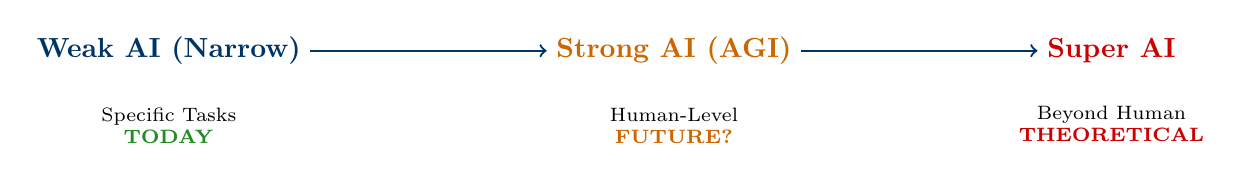
\begin{tikzpicture}
        \node[font=\bfseries, text=ukhblue] (weak) {Weak AI (Narrow)};
        \node[right=3cm of weak, font=\bfseries, text=orange!80!black] (strong) {Strong AI (AGI)};
        \node[right=3cm of strong, font=\bfseries, text=alertred] (super) {Super AI};
        
        \node[below=0.3cm of weak, align=center, font=\scriptsize] {Specific Tasks\\{\color{forestgreen}\textbf{TODAY}}};
        \node[below=0.3cm of strong, align=center, font=\scriptsize] {Human-Level\\{\color{orange!80!black}\textbf{FUTURE?}}};
        \node[below=0.3cm of super, align=center, font=\scriptsize] {Beyond Human\\{\color{alertred}\textbf{THEORETICAL}}};
        
        \draw[->, thick, ukhblue] (weak) -- (strong);
        \draw[->, thick, ukhblue] (strong) -- (super);
    \end{tikzpicture}
    
    \vspace{1em}
    
    \begin{concept_box}{Important}
        \textbf{ChatGPT, Claude, Gemini} --- all current AI tools are \textbf{Weak AI}. They excel at specific tasks but don't truly ``understand'' like humans do.
    \end{concept_box}
\end{frame}

\begin{frame}{AI History: Key Milestones}
    \begin{columns}[t]
        \column{0.48\textwidth}
        \begin{concept_box}{1960s: First Steps}
            \small
            \begin{itemize}
                \item \textbf{ELIZA (1964)} --- First chatbot (therapist)
                \item \textbf{Shakey (1966)} --- First mobile robot
            \end{itemize}
        \end{concept_box}
        
        \vspace{0.3em}
        
        \begin{info_box}{1990s: AI Gets Smart}
            \small
            \begin{itemize}
                \item \textbf{Deep Blue (1997)} --- Beat chess champion
                \item \textbf{Google Search} --- Web indexing
            \end{itemize}
        \end{info_box}
        
        \column{0.48\textwidth}
        \begin{example_box}{2010s: Deep Learning}
            \small
            \begin{itemize}
                \item \textbf{AlexNet (2012)} --- Image recognition
                \item \textbf{AlphaGo (2016)} --- Beat Go champion
            \end{itemize}
        \end{example_box}
        
        \vspace{0.3em}
        
        \begin{warning_box}{2020s: The Revolution}
            \small
            \begin{itemize}
                \item \textbf{ChatGPT (2022)} --- AI writes like humans
                \item \textbf{Gemini/Claude} --- Multimodal AI
            \end{itemize}
        \end{warning_box}
    \end{columns}
\end{frame}

% ============================================================================
% SECTION 1.5: AI TOOLS OVERVIEW
% ============================================================================
\section{AI Tools for Researchers}

\begin{frame}{AI Tools Overview}
    \centering
    \small
    \begin{tabular}{llll}
        \toprule
        \textbf{Tool} & \textbf{What It Does} & \textbf{Cost} & \textbf{URL} \\
        \midrule
        \textbf{ChatGPT} & General AI, coding, file analysis & Free / \$20/mo & chat.openai.com \\
        \textbf{Claude} & Long docs, academic writing & Free / \$20/mo & claude.ai \\
        \textbf{Gemini} & Images, Google integration & Free / \$20/mo & gemini.google.com \\
        \textbf{DeepSeek} & Free GPT-4 alternative & \textbf{Free!} & chat.deepseek.com \\
        \textbf{Perplexity} & Web search with citations & Free / \$20/mo & perplexity.ai \\
        \bottomrule
    \end{tabular}
    
    \vspace{0.8em}
    
    \begin{info_box}{Key Point}
        \small Each tool has unique strengths. Smart researchers use \textbf{multiple tools} for different tasks!
    \end{info_box}
\end{frame}

\begin{frame}{Key Features to Know}
    \begin{columns}[t]
        \column{0.48\textwidth}
        \begin{concept_box}{Deep Research Mode}
            \small Available in ChatGPT \& Gemini. AI browses the web, analyzes sources, and writes reports with citations.
        \end{concept_box}
        
        \vspace{0.3em}
        
        \begin{info_box}{NotebookLM (FREE)}
            \small Google's AI for your papers. Upload docs $\to$ get AI podcasts, summaries, Q\&A!\\
            \textbf{URL:} notebooklm.google.com
        \end{info_box}
        
        \column{0.48\textwidth}
        \begin{warning_box}{z.ai by Zotero}
            \small AI integrated with Zotero. Chat with your library, summarize papers.\\
            \textbf{URL:} z.ai
        \end{warning_box}
        
        \vspace{0.3em}
        
        \begin{example_box}{DeepSeek (FREE)}
            \small Chinese AI rivaling ChatGPT. Completely free with no limits!
        \end{example_box}
    \end{columns}
\end{frame}

% ============================================================================
% SECTION 2: PROMPT ENGINEERING
% ============================================================================
\section{Prompt Engineering Fundamentals}

\begin{frame}{What is Prompt Engineering?}
    \begin{info_box}{Definition}
        \textbf{Prompt Engineering} is the art and science of crafting effective instructions to get the best possible output from AI systems.
    \end{info_box}
    
    \vspace{0.5em}
    
    \begin{columns}
        \column{0.5\textwidth}
        \textbf{Why It Matters:}
        \begin{itemize}
            \item Same AI, different prompts $\to$ vastly different results
            \item Good prompts save time and improve quality
            \item Essential skill for researchers
        \end{itemize}
        
        \column{0.5\textwidth}
        \textbf{Key Insight:}
        \begin{quote_box}
            ``AI doesn't read your mind. The quality of output depends entirely on the quality of your input.''
        \end{quote_box}
    \end{columns}
\end{frame}

\begin{frame}{The CARE Framework}
    \begin{info_box}{A Simple Framework for Effective Prompts}
        \textbf{C}ontext --- \textbf{A}ction --- \textbf{R}ole --- \textbf{E}xpectations
    \end{info_box}
    
    \vspace{1em}
    
    \begin{columns}[t]
        \column{0.24\textwidth}
        \begin{concept_box}{\textbf{C}ontext}
            \small Background, domain, constraints
        \end{concept_box}
        
        \column{0.24\textwidth}
        \begin{concept_box}{\textbf{A}ction}
            \small What to do (verb)
        \end{concept_box}
        
        \column{0.24\textwidth}
        \begin{concept_box}{\textbf{R}ole}
            \small Persona to adopt
        \end{concept_box}
        
        \column{0.24\textwidth}
        \begin{concept_box}{\textbf{E}xpectations}
            \small Format, length, style
        \end{concept_box}
    \end{columns}
\end{frame}

\begin{frame}{CARE Framework: Example}
    \begin{example_box}{Example Prompt Using CARE}
        \small
        ``\textbf{[Role]} Act as an academic researcher in digital marketing.
        
        \textbf{[Context]} I'm writing a literature review on social media advertising.
        
        \textbf{[Action]} Analyze the key themes in this field from 2020-2024.
        
        \textbf{[Expectations]} Present findings in a table with columns: Theme, Key Authors, Gaps.''
    \end{example_box}
    
    \vspace{0.5em}
    
    \begin{info_box}{Result}
        \small This structured prompt will generate academic-quality, organized output rather than generic text.
    \end{info_box}
\end{frame}

\begin{frame}{Professional Personas}
    \begin{info_box}{Shifting AI's Tone}
        Using ``Act as...'' prompts dramatically changes the quality and style of AI responses.
    \end{info_box}
    
    \vspace{0.5em}
    
    \begin{columns}[t]
        \column{0.5\textwidth}
        \textbf{For Academic Writing:}
        \begin{itemize}
            \item ``Act as an academic researcher...''
            \item ``Act as a peer reviewer for a journal...''
            \item ``Act as a thesis supervisor...''
            \item ``Act as a methodologist...''
        \end{itemize}
        
        \column{0.5\textwidth}
        \textbf{For Technical Tasks:}
        \begin{itemize}
            \item ``Act as a statistician using SPSS...''
            \item ``Act as a Python data analyst...''
            \item ``Act as a LaTeX expert...''
            \item ``Act as a Harvard citation specialist...''
        \end{itemize}
    \end{columns}
    
    \vspace{0.5em}
    
    \begin{warning_box}{Remember}
        \small Personas help get better output, but you must still verify all information!
    \end{warning_box}
\end{frame}

\begin{frame}{Context: Setting the Stage}
    \begin{info_box}{What is Context?}
        Background information that helps AI understand your situation, field, and constraints.
    \end{info_box}
    
    \vspace{0.5em}
    
    \begin{columns}[t]
        \column{0.5\textwidth}
        \textbf{What to Include:}
        \begin{itemize}
            \item Your academic field/discipline
            \item The specific topic or problem
            \item Relevant constraints (word limit, deadline)
            \item Your level (PhD, Master's, etc.)
        \end{itemize}
        
        \column{0.5\textwidth}
        \textbf{Examples:}
        \begin{itemize}
            \item ``I'm a Master's student in Marketing...''
            \item ``I'm writing a literature review on...''
            \item ``This is for a 5000-word thesis chapter...''
            \item ``I'm researching in the Kurdish context...''
        \end{itemize}
    \end{columns}
    
    \vspace{0.5em}
    
    \begin{concept_box}{Why It Matters}
        \small More context = more relevant output. AI can't read your mind!
    \end{concept_box}
\end{frame}

\begin{frame}{Action: What Do You Want?}
    \begin{info_box}{What is Action?}
        The specific task you want the AI to perform. Use clear, strong verbs.
    \end{info_box}
    
    \vspace{0.5em}
    
    \begin{columns}[t]
        \column{0.5\textwidth}
        \textbf{Strong Action Verbs:}
        \begin{itemize}
            \item \textbf{Analyze} --- Examine in detail
            \item \textbf{Compare} --- Find differences
            \item \textbf{Summarize} --- Condense info
            \item \textbf{Generate} --- Create content
        \end{itemize}
        
        \column{0.5\textwidth}
        \textbf{More Action Verbs:}
        \begin{itemize}
            \item \textbf{Identify} --- Find items
            \item \textbf{Explain} --- Clarify concepts
            \item \textbf{Organize} --- Structure content
            \item \textbf{Critique} --- Evaluate critically
        \end{itemize}
    \end{columns}
    
    \vspace{0.3em}
    
    \begin{warning_box}{Avoid Vague Actions}
        \small ``Write about...'' $\to$ ``Analyze the key themes in...''
    \end{warning_box}
\end{frame}

\begin{frame}{Expectations: Define the Output}
    \begin{info_box}{What are Expectations?}
        The format, length, style, and structure you want in the response.
    \end{info_box}
    
    \vspace{0.5em}
    
    \begin{columns}[t]
        \column{0.5\textwidth}
        \textbf{Format Options:}
        \begin{itemize}
            \item ``Present as a table with columns...''
            \item ``Use bullet points for each item...''
            \item ``Write in academic paragraph form...''
            \item ``Create a numbered list of 5 items...''
        \end{itemize}
        
        \column{0.5\textwidth}
        \textbf{Style \& Length:}
        \begin{itemize}
            \item ``Use formal academic language...''
            \item ``Keep each point to 2-3 sentences...''
            \item ``Include citations where possible...''
            \item ``Be concise but comprehensive...''
        \end{itemize}
    \end{columns}
    
    \vspace{0.5em}
    
    \begin{example_box}{Complete Expectation Example}
        \small ``Present findings in a table with 4 columns: Author, Year, Key Finding, Methodology. Include 10-15 relevant papers.''
    \end{example_box}
\end{frame}

\begin{frame}{Advanced Prompt Techniques}
    \begin{columns}[t]
        \column{0.5\textwidth}
        \begin{concept_box}{Negative Prompts}
            \scriptsize ``Do NOT include generic advice. Avoid clichés.''
        \end{concept_box}
        
        \vspace{0.2em}
        
        \begin{info_box}{Chain-of-Thought}
            \scriptsize ``Think step by step. First analyze X, then compare Y.''
        \end{info_box}
        
        \vspace{0.2em}
        
        \begin{example_box}{Few-Shot Examples}
            \scriptsize Provide 1-2 examples of desired output.
        \end{example_box}
        
        \column{0.5\textwidth}
        \begin{concept_box}{Context Dump}
            \scriptsize Upload docs, paste abstracts, provide background.
        \end{concept_box}
        
        \vspace{0.2em}
        
        \begin{info_box}{Ask to Clarify}
            \scriptsize ``Ask me clarifying questions before proceeding.''
        \end{info_box}
        
        \vspace{0.2em}
        
       
    \end{columns}
\end{frame}

\begin{frame}{Good vs. Bad Prompts}
    \begin{columns}
        \column{0.48\textwidth}
        \begin{warning_box}{Bad Prompt \faTimesCircle}
            \small
            ``Write about digital marketing.''
            
            \vspace{0.5em}
            \textbf{Problems:}
            \begin{itemize}
                \item Too vague
                \item No context or purpose
                \item No format specified
                \item Will get generic output
            \end{itemize}
        \end{warning_box}
        
        \column{0.48\textwidth}
        \begin{concept_box}{Good Prompt \faCheckCircle}
            \small
            ``Act as a marketing researcher. I'm a Master's student studying the impact of influencer marketing on Gen Z purchasing behavior in Kurdistan. Generate 5 potential research gaps with supporting rationale and suggested methodologies.''
            
            \vspace{0.3em}
            \textbf{Includes:}
            Role, Context, Specifics, Format
        \end{concept_box}
    \end{columns}
\end{frame}

\begin{frame}{Prompt Engineering Tips}
    \begin{columns}[t]
        \column{0.5\textwidth}
        \textbf{\faLightbulb\ Best Practices:}
        \begin{enumerate}
            \item \textbf{Be Specific} --- Include details, constraints, examples
            \item \textbf{Iterate} --- Refine based on output
            \item \textbf{Break Down} --- Complex tasks into steps
            \item \textbf{Request Format} --- Tables, bullet points, etc.
            \item \textbf{Ask for Sources} --- ``Include citations''
        \end{enumerate}
        
        \column{0.5\textwidth}
        \textbf{\faExclamationTriangle\ Common Mistakes:}
        \begin{enumerate}
            \item Being too vague or broad
            \item Not specifying the audience
            \item Forgetting to ask for sources
            \item Accepting first output without iteration
            \item Not providing examples
        \end{enumerate}
    \end{columns}
    
    \vspace{0.5em}
    
    \begin{info_box}{Pro Tip}
        \small Always end with: ``If you need any clarification, ask me before proceeding.''
    \end{info_box}
\end{frame}

% ============================================================================
% SECTION 3: AI FOR RESEARCH TASKS
% ============================================================================
\section{AI for Research Tasks}

\begin{frame}{11 Research Tasks AI Can Assist With}
    \begin{columns}[t]
        \column{0.32\textwidth}
        \begin{concept_box}{\small \faSearch\ Planning}
            \scriptsize
            \begin{enumerate}
                \item Gap Finding
                \item Title Generation
                \item Research Outline
                \item Research Questions
            \end{enumerate}
        \end{concept_box}
        
        \column{0.32\textwidth}
        \begin{info_box}{\small \faBook\ Research}
            \scriptsize
            \begin{enumerate}
                \setcounter{enumi}{4}
                \item Literature Review
                \item Novel Concepts
                \item Article Comparison
            \end{enumerate}
        \end{info_box}
        
        \column{0.32\textwidth}
        \begin{example_box}{\small \faChartBar\ Analysis}
            \scriptsize
            \begin{enumerate}
                \setcounter{enumi}{7}
                \item Data Analysis
                \item Visualization
                \item References
                \item LaTeX Formatting
            \end{enumerate}
        \end{example_box}
    \end{columns}
    
    \vspace{0.5em}
    
    \begin{warning_box}{Critical Reminder}
        \small AI is an \textbf{assistant}, not a replacement. You remain the \textbf{author} and are responsible for all content.
    \end{warning_box}
\end{frame}

% ==================== TASK 1: GAP FINDING ====================
\begin{frame}{Task 1: Finding the Research Gap}
    \begin{info_box}{What is a Research Gap?}
        An unexplored or under-researched area in existing literature where your research can contribute new knowledge.
    \end{info_box}
    
    \vspace{0.5em}
    
    \begin{columns}[t]
        \column{0.5\textwidth}
        \textbf{Why It Matters:}
        \begin{itemize}
            \item Justifies your research
            \item Shows originality
            \item Guides your focus
            \item Required in thesis proposals
        \end{itemize}
        
        \column{0.5\textwidth}
        \textbf{AI Can Help By:}
        \begin{itemize}
            \item Analyzing recent papers
            \item Identifying understudied areas
            \item Suggesting research questions
            \item Finding dimension combinations
        \end{itemize}
    \end{columns}
\end{frame}

\begin{frame}{Task 1: Gap Finding --- Live Demo Prompt}
    \begin{prompt_box}{Copy This Prompt}
        \small
        ``Act as an academic researcher specializing in \textbf{Digital Marketing}. I am a Master's student interested in studying \textbf{social media marketing in the Kurdistan Region}.

        Analyze recent literature (2020-2024) and identify 5 potential research gaps. For each gap, provide:
        \begin{itemize}
            \item The gap description (what is missing)
            \item Why it matters (significance)
            \item 2-3 potential research questions
            \item Suggested methodology
        \end{itemize}
        
        Focus on understudied contexts, populations, or variable combinations. Present in a structured format with clear headings.''
    \end{prompt_box}
\end{frame}

% ==================== TASK 2: RESEARCH OUTLINE ====================
\begin{frame}{Task 2: Research Outline Generation}
    \begin{info_box}{What is Research Outline Generation?}
        Using AI to create a complete, structured thesis or dissertation outline based on your research title.
    \end{info_box}
    
    \vspace{0.5em}
    
    \begin{columns}[t]
        \column{0.5\textwidth}
        \textbf{Why It Matters:}
        \begin{itemize}
            \item Provides research roadmap
            \item Ensures logical structure
            \item Saves planning time
            \item Identifies all sections needed
        \end{itemize}
        
        \column{0.5\textwidth}
        \textbf{AI Can Generate:}
        \begin{itemize}
            \item Chapter breakdowns
            \item Section headings
            \item Content descriptions
            \item Word count estimates
        \end{itemize}
    \end{columns}
\end{frame}

\begin{frame}{Task 2: Research Outline --- Live Demo Prompt}
    \begin{prompt_box}{Copy This Prompt}
        \small
        ``Act as an academic thesis advisor. Based on the following research title, generate a complete Master's thesis outline:

        \textbf{Title:} [PASTE YOUR TITLE HERE]
        
        Provide a comprehensive outline including:
        \begin{itemize}
            \item All chapters with numbered sections/subsections
            \item Brief description of each section's content
            \item Suggested word count per chapter
            \item Key components for Literature Review \& Methodology
            \item Expected tables/figures for each chapter
        \end{itemize}
        
        Format as a hierarchical structure (1, 1.1, 1.1.1). Total target: 15,000-20,000 words.''
    \end{prompt_box}
\end{frame}

% ==================== TASK 3: RESEARCH QUESTIONS ====================
\begin{frame}{Task 3: Research Questions \& Hypotheses}
    \begin{info_box}{What are Research Questions \& Hypotheses?}
        Clear, testable statements that guide your entire research study and methodology.
    \end{info_box}
    
    \vspace{0.5em}
    
    \begin{columns}[t]
        \column{0.5\textwidth}
        \textbf{Why It Matters:}
        \begin{itemize}
            \item Focuses your research
            \item Determines methodology
            \item Required in proposals
            \item Guides data collection
        \end{itemize}
        
        \column{0.5\textwidth}
        \textbf{AI Can Generate:}
        \begin{itemize}
            \item Main RQ + sub-questions
            \item Null \& alternative hypotheses
            \item Variable relationships
            \item Testable statements
        \end{itemize}
    \end{columns}
\end{frame}

\begin{frame}{Task 3: Research Questions --- Live Demo Prompt}
    \begin{prompt_box}{Copy This Prompt}
        \small
        ``Act as a research methodology expert. Based on my research title:

        \textbf{Title:} [PASTE YOUR TITLE HERE]
        
        Generate comprehensive research questions and hypotheses:
        \begin{itemize}
            \item 1 Main Research Question (broad, overarching)
            \item 3-5 Specific Sub-Questions (measurable, focused)
            \item Corresponding Null \& Alternative Hypotheses for each
            \item Identify IV, DV, and mediating/moderating variables
        \end{itemize}
        
        Format: RQ1, RQ1a, RQ1b... with H0/H1 pairs. Ensure all are testable and aligned with quantitative/qualitative methodology.''
    \end{prompt_box}
\end{frame}

% ==================== TASK 4: TITLE GENERATION ====================
\begin{frame}{Task 4: Title \& Idea Generation}
    \begin{info_box}{What is Title Generation?}
        Using AI to brainstorm research titles, refine topic scope, and generate thesis ideas.
    \end{info_box}
    
    \vspace{0.5em}
    
    \begin{columns}[t]
        \column{0.5\textwidth}
        \textbf{Why It Matters:}
        \begin{itemize}
            \item Saves brainstorming time
            \item Explores different angles
            \item Helps narrow your focus
            \item Generates variations
        \end{itemize}
        
        \column{0.5\textwidth}
        \textbf{AI Can Help By:}
        \begin{itemize}
            \item Generating 10+ title options
            \item Varying methodologies
            \item Suggesting variables
            \item Explaining contributions
        \end{itemize}
    \end{columns}
    
    \vspace{0.3em}
    
    \begin{warning_box}{Remember}
        \small Use AI titles as \textbf{starting points}. Always refine with your supervisor!
    \end{warning_box}
\end{frame}

\begin{frame}{Task 4: Title Generation --- Live Demo Prompt}
    \begin{prompt_box}{Copy This Prompt}
        \small
        ``Act as a thesis supervisor at a business school. Generate 10 potential research titles for a Master's thesis in \textbf{Marketing} focusing on \textbf{digital advertising effectiveness}.

        Requirements for each title:
        \begin{itemize}
            \item Be specific and clearly researchable
            \item Include independent and dependent variables
            \item Vary the methodological approaches (quantitative, qualitative, mixed)
            \item Consider the Kurdistan Region context where applicable
        \end{itemize}
        
        For each title, provide a 2-sentence explanation of the potential contribution. Present as a numbered list.''
    \end{prompt_box}
\end{frame}

% ==================== TASK 5: LITERATURE REVIEW ====================
\begin{frame}{Task 5: Literature Review Assistance}
    \begin{info_box}{What is Literature Review Assistance?}
        Using AI to organize, summarize, and find patterns across multiple research papers.
    \end{info_box}
    
    \vspace{0.5em}
    
    \begin{columns}[t]
        \column{0.5\textwidth}
        \textbf{What AI Can Do:}
        \begin{itemize}
            \item Summarize papers
            \item Organize by themes
            \item Track chronological trends
            \item Compare methodologies
        \end{itemize}
        
        \column{0.5\textwidth}
        \textbf{What AI Cannot Do:}
        \begin{itemize}
            \item Access real databases
            \item Verify citations
            \item Replace critical reading
            \item Guarantee accuracy
        \end{itemize}
    \end{columns}
    
    \vspace{0.3em}
    
    \begin{warning_box}{Critical Warning}
        \small AI may generate \textbf{fake citations}! Always verify using Google Scholar.
    \end{warning_box}
\end{frame}

\begin{frame}{Task 5: Literature Review --- Live Demo Prompt}
    \begin{prompt_box}{Copy This Prompt}
        \small
        ``Act as an academic researcher. I am conducting a literature review on \textbf{influencer marketing and consumer purchase intentions}.

        Analyze the key themes in this research area from 2020-2024. For each theme:
        \begin{itemize}
            \item Identify the main focus and scope
            \item List key authors and seminal papers
            \item Describe common methodologies used
            \item Note any gaps or inconsistencies in findings
        \end{itemize}
        
        Present your findings in a table with columns: Theme Name, Key Focus, Main Authors, Common Methods, Research Gaps. Include at least 5 themes.''
    \end{prompt_box}
\end{frame}

% ==================== TASK 6: NOVEL CONCEPTS ====================
\begin{frame}{Task 6: Novel Concept Generation}
    \begin{info_box}{What is Novel Concept Generation?}
        Using AI to help create new definitions, frameworks, or conceptual combinations for original contributions.
    \end{info_box}
    
    \vspace{0.5em}
    
    \begin{columns}[t]
        \column{0.5\textwidth}
        \textbf{Types of Novelty:}
        \begin{itemize}
            \item New definitions
            \item Combined frameworks
            \item Extended theories
            \item New constructs
        \end{itemize}
        
        \column{0.5\textwidth}
        \textbf{AI Can Help By:}
        \begin{itemize}
            \item Combining concepts
            \item Suggesting terminology
            \item Providing justification
            \item Comparing to existing work
        \end{itemize}
    \end{columns}
    
    \vspace{0.3em}
    
    \begin{warning_box}{Critical}
        \small You MUST rewrite AI-generated concepts in your own words. Never copy-paste!
    \end{warning_box}
\end{frame}

\begin{frame}{Task 6: Novel Concepts --- Live Demo Prompt}
    \begin{prompt_box}{Copy This Prompt}
        \small
        ``Act as a theoretical researcher. I want to create a novel concept that combines \textbf{social media marketing} with \textbf{cultural identity theory} in the context of the Kurdistan Region.

        Develop:
        \begin{itemize}
            \item A new term or concept name
            \item A formal academic definition (2-3 sentences)
            \item Theoretical justification explaining why this combination is meaningful
            \item How it differs from existing concepts in the literature
            \item 3 potential research questions using this concept
        \end{itemize}
        
        Use formal academic journal language throughout.''
    \end{prompt_box}
\end{frame}

% ==================== TASK 7: ARTICLE COMPARISON ====================
\begin{frame}{Task 7: Article Comparison}
    \begin{info_box}{What is Article Comparison?}
        Using AI to systematically compare multiple research papers across key dimensions.
    \end{info_box}
    
    \vspace{0.5em}
    
    \begin{columns}[t]
        \column{0.5\textwidth}
        \textbf{Comparison Dimensions:}
        \begin{itemize}
            \item Research objectives
            \item Methodology/sample
            \item Theoretical framework
            \item Key findings
        \end{itemize}
        
        \column{0.5\textwidth}
        \textbf{Use Cases:}
        \begin{itemize}
            \item Contrast old vs. new studies
            \item Compare methodologies
            \item Find conflicting findings
            \item Build synthesis
        \end{itemize}
    \end{columns}
    
    \vspace{0.3em}
    
    \begin{concept_box}{Pro Tip}
        \small Upload PDFs or paste abstracts directly into ChatGPT or Claude for accurate comparison.
    \end{concept_box}
\end{frame}

\begin{frame}{Task 7: Article Comparison --- Live Demo Prompt}
    \begin{prompt_box}{Copy This Prompt}
        \small
        ``Act as an academic reviewer. I will provide you with two research paper abstracts. Compare them systematically on these dimensions:

        \begin{itemize}
            \item Research objectives and questions
            \item Theoretical/conceptual framework
            \item Methodology and sample characteristics
            \item Key findings and conclusions
            \item Limitations acknowledged
        \end{itemize}
        
        Present your analysis in two formats:
        1. A comparison table with the dimensions as rows
        2. A 5-sentence synthesis paragraph highlighting key similarities and differences
        
        [PASTE YOUR TWO ABSTRACTS HERE]''
    \end{prompt_box}
\end{frame}

% ==================== TASK 8: DATA ANALYSIS ====================
\begin{frame}{Task 8: Data Analysis Assistance}
    \begin{info_box}{What is Data Analysis Assistance?}
        Using AI to help with statistical test selection, code generation, and results interpretation.
    \end{info_box}
    
    \vspace{0.5em}
    
    \begin{columns}[t]
        \column{0.5\textwidth}
        \textbf{AI Can Help With:}
        \begin{itemize}
            \item Choosing the right test
            \item Writing SPSS/Python/R code
            \item Interpreting outputs
            \item Creating tables
        \end{itemize}
        
        \column{0.5\textwidth}
        \textbf{Tools to Use:}
        \begin{itemize}
            \item ChatGPT Code Interpreter
            \item Claude with data upload
            \item Gemini for analysis
            \item Specialized AI tools
        \end{itemize}
    \end{columns}
    
    \vspace{0.3em}
    
    \begin{warning_box}{Important}
        \small You must understand the statistical concepts. AI helps with execution, not learning!
    \end{warning_box}
\end{frame}

\begin{frame}{Task 8: Data Analysis --- Live Demo Prompt}
    \begin{prompt_box}{Copy This Prompt}
        \small
        ``Act as a statistical consultant. I have survey data with these variables:
        \begin{itemize}
            \item Independent: Social Media Usage (Likert 1-5)
            \item Dependent: Purchase Intention (Likert 1-5)
            \item Moderator: Age Group (categorical: 18-25, 26-35, 36+)
        \end{itemize}
        
        I want to test if social media usage affects purchase intention, and if age moderates this relationship.
        
        Provide:
        1. The appropriate statistical test and why
        2. SPSS syntax to run this analysis
        3. How to interpret the key outputs
        4. How to report the results in APA format''
    \end{prompt_box}
\end{frame}

% ==================== TASK 9: VISUALIZATION ====================
\begin{frame}{Task 9: Visualization \& Posters}
    \begin{info_box}{What is Visualization Assistance?}
        Using AI to generate charts, graphs, diagrams, posters, and even audio/video explanations.
    \end{info_box}
    
    \vspace{0.5em}
    
    \begin{columns}[t]
        \column{0.5\textwidth}
        \textbf{What AI Can Create:}
        \begin{itemize}
            \item Charts \& graphs (bar, line, scatter)
            \item Research model diagrams
            \item Conference posters
            \item Audio podcasts \& summaries
        \end{itemize}
        
        \column{0.5\textwidth}
        \textbf{Key Tools (Google):}
        \begin{itemize}
            \item \textbf{Gemini} --- Images \& figures
            \item \textbf{NotebookLM} --- Podcasts \& explanations
            \item ChatGPT --- Python code
            \item Canva AI --- Poster design
        \end{itemize}
    \end{columns}
    
    \vspace{0.3em}
    
    \begin{concept_box}{NotebookLM by Google}
        \small Upload your papers and generate: audio podcasts, deep-dive summaries, explanation videos, and interactive Q\&A about your research!
    \end{concept_box}
\end{frame}

\begin{frame}{Task 9: Visualization --- Live Demo Prompt}
    \begin{prompt_box}{Gemini: Generate Research Figure}
        \small
        ``Create a professional visualization showing the relationship between \textbf{Social Media Engagement} and \textbf{Brand Loyalty} across three age groups.

        Requirements:
        \begin{itemize}
            \item Use a grouped bar chart style
            \item Academic-appropriate colors (blues, grays)
            \item Include proper labels and legend
            \item Make it suitable for a journal article
        \end{itemize}''
    \end{prompt_box}
    
    \vspace{0.3em}
    
    \begin{info_box}{NotebookLM: Generate Podcast}
        \small Upload your thesis chapter or literature review $\to$ Click ``Audio Overview'' $\to$ Get a 10-minute podcast summary of your research!
    \end{info_box}
\end{frame}

% ==================== TASK 10: REFERENCES ====================
\begin{frame}{Task 10: Reference Management}
    \begin{info_box}{What is Reference Management?}
        Using AI to format, convert, and organize citations in the correct style.
    \end{info_box}
    
    \vspace{0.5em}
    
    \begin{columns}[t]
        \column{0.5\textwidth}
        \textbf{AI Can Help With:}
        \begin{itemize}
            \item Converting citation styles
            \item Formatting references
            \item Finding missing info
            \item Alphabetizing lists
        \end{itemize}
        
        \column{0.5\textwidth}
        \textbf{Common Styles:}
        \begin{itemize}
            \item Harvard (SUE standard)
            \item APA 7th Edition
            \item IEEE, Chicago, MLA
            \item Journal-specific styles
        \end{itemize}
    \end{columns}
    
    \vspace{0.3em}
    
    \begin{concept_box}{SUE Standard}
        \small Harvard referencing is the official style at Salahaddin University.
    \end{concept_box}
\end{frame}

\begin{frame}{Task 10: References --- Live Demo Prompt}
    \begin{prompt_box}{Copy This Prompt}
        \small
        ``Act as a citation expert specializing in Harvard referencing style. Convert the following references to Harvard format:

        [PASTE YOUR REFERENCES HERE]

        For each reference:
        \begin{itemize}
            \item Format according to Harvard style guidelines
            \item Ensure author names are: Surname, Initial.
            \item Italicize journal/book titles appropriately
            \item Include DOI or URL where available
        \end{itemize}
        
        Then alphabetize the complete list, remove any duplicates, and flag any entries with missing information.''
    \end{prompt_box}
\end{frame}

% ==================== TASK 11: LATEX ====================
\begin{frame}{Task 11: LaTeX Formatting}
    \begin{info_box}{What is LaTeX?}
        A professional document preparation system used for academic papers, especially those with equations, tables, and figures.
    \end{info_box}
    
    \vspace{0.5em}
    
    \begin{columns}[t]
        \column{0.5\textwidth}
        \textbf{Why Use LaTeX:}
        \begin{itemize}
            \item Professional typesetting
            \item Automatic formatting
            \item Better equations
            \item Required by journals
        \end{itemize}
        
        \column{0.5\textwidth}
        \textbf{AI Can Help With:}
        \begin{itemize}
            \item Converting Word to LaTeX
            \item Creating tables/figures
            \item Writing TikZ diagrams
            \item Debugging errors
        \end{itemize}
    \end{columns}
\end{frame}

\begin{frame}{Task 11: LaTeX --- Live Demo Prompt}
    \begin{prompt_box}{Copy This Prompt}
        \small
        ``Convert the following text into a professional LaTeX document:

        [PASTE YOUR TEXT HERE]

        Requirements:
        \begin{itemize}
            \item Use the article document class, 12pt font
            \item Include a title, author, and abstract section
            \item Format any tables using booktabs package
            \item Number sections and subsections automatically
            \item Add proper figure placeholders with captions
        \end{itemize}
        
        Provide the complete LaTeX code that I can compile directly in Overleaf.''
    \end{prompt_box}
\end{frame}

% ============================================================================
% SECTION 4: AI LIMITATIONS & HALLUCINATIONS
% ============================================================================
\section{AI Hallucinations \& Limitations}

\begin{frame}{What are AI Hallucinations?}
    \begin{warning_box}{Definition}
        \textbf{AI Hallucination}: When an AI generates information that is false, fabricated, or not grounded in reality --- but presents it confidently as fact.
    \end{warning_box}
    
    \vspace{0.5em}
    
    \begin{columns}[t]
        \column{0.5\textwidth}
        \textbf{Common Hallucination Types:}
        \begin{itemize}
            \item \textbf{Fake Citations} --- Non-existent papers
            \item \textbf{Wrong Authors} --- Misattributed work
            \item \textbf{Invented Statistics} --- Made-up numbers
            \item \textbf{False Facts} --- Incorrect information
        \end{itemize}
        
        \column{0.5\textwidth}
        \textbf{Why It Happens:}
        \begin{itemize}
            \item AI predicts ``likely'' text
            \item No real understanding
            \item Training data gaps
            \item Pattern matching, not reasoning
        \end{itemize}
    \end{columns}
\end{frame}

\begin{frame}{Hallucination Examples}
    \begin{columns}
        \column{0.48\textwidth}
        \begin{warning_box}{Fake Citation}
            \scriptsize
            \textbf{AI Output:}\\
            ``Smith, J. \& Johnson, M. (2023). The Impact of Social Media on Consumer Behavior. \textit{Journal of Marketing Research}, 45(2), 123-145.''
            
            \vspace{0.3em}
            \textbf{Reality:} This paper doesn't exist. The authors, volume, and page numbers are fabricated.
        \end{warning_box}
        
        \column{0.48\textwidth}
        \begin{warning_box}{Invented Statistics}
            \scriptsize
            \textbf{AI Output:}\\
            ``According to a 2024 UNESCO report, 78\% of universities in the Middle East have adopted AI policies.''
            
            \vspace{0.3em}
            \textbf{Reality:} No such report exists. The percentage is made up.
        \end{warning_box}
    \end{columns}
    
    \vspace{0.5em}
    
    \begin{concept_box}{The Danger}
        \small AI hallucinations can destroy your academic credibility. One fake citation in a thesis can have serious consequences.
    \end{concept_box}
\end{frame}

\begin{frame}{How to Detect and Prevent Hallucinations}
    \begin{columns}[t]
        \column{0.5\textwidth}
        \textbf{\faSearch\ Detection Methods:}
        \begin{enumerate}
            \item \textbf{Verify Citations} --- Check Google Scholar
            \item \textbf{Cross-Reference} --- Use multiple sources
            \item \textbf{Check DOIs} --- Real papers have DOIs
            \item \textbf{Read Abstracts} --- Confirm content matches
            \item \textbf{Be Skeptical} --- Question confident claims
        \end{enumerate}
        
        \column{0.5\textwidth}
        \textbf{\faShield*\ Prevention Strategies:}
        \begin{enumerate}
            \item Ask AI to ``only cite verifiable sources''
            \item Request URLs/DOIs with citations
            \item Use AI tools with web access
            \item Treat all outputs as drafts
            \item Never submit without verification
        \end{enumerate}
    \end{columns}
    
    \vspace{0.5em}
    
    \begin{info_box}{Golden Rule}
        \small \textbf{Trust, but verify.} AI can help you find sources, but YOU must confirm they exist and say what AI claims.
    \end{info_box}
\end{frame}

\begin{frame}{Other AI Limitations}
    \begin{columns}[t]
        \column{0.5\textwidth}
        \begin{warning_box}{Technical Issues}
            \small
            \begin{itemize}
                \item \textbf{Knowledge Cutoff} --- Outdated info
                \item \textbf{No Understanding} --- Pattern matching
                \item \textbf{Context Limits} --- Forgets context
                \item \textbf{Math Errors} --- Miscalculates
            \end{itemize}
        \end{warning_box}
        
        \column{0.5\textwidth}
        \begin{warning_box}{Content Issues}
            \small
            \begin{itemize}
                \item \textbf{Bias} --- Training data biases
                \item \textbf{Inconsistency} --- Varies outputs
                \item \textbf{No Judgment} --- Can't evaluate
                \item \textbf{Cultural Gaps} --- Western-centric
            \end{itemize}
        \end{warning_box}
    \end{columns}
    
    \vspace{0.3em}
    
    \begin{quote_box}
        ``AI is a knowledgeable but unreliable colleague. Great for brainstorming, dangerous for facts.''
    \end{quote_box}
\end{frame}

% ============================================================================
% SECTION 5: ETHICS & ACADEMIC INTEGRITY
% ============================================================================
\section{Ethics \& Academic Integrity}

\begin{frame}{AI as an Assistant, Not a Replacement}
    \begin{info_box}{The Core Philosophy}
        AI should \textbf{assist} your research, not \textbf{replace} your thinking. You remain the \textbf{author} and \textbf{intellectual owner} of your work.
    \end{info_box}
    
    \vspace{0.5em}
    
    \centering
    \begin{tikzpicture}
        \node[draw=forestgreen, fill=green!10, rounded corners, text width=5cm, align=center] (good) {
            \textbf{\faCheckCircle\ Good Use}\\
            \small Brainstorming, outlining, editing, formatting, finding sources
        };
        
        \node[draw=alertred, fill=red!10, rounded corners, text width=5cm, align=center, right=1cm of good] (bad) {
            \textbf{\faTimesCircle\ Bad Use}\\
            \small Writing entire sections, copying without review, fabricating data
        };
    \end{tikzpicture}
    
    \vspace{0.5em}
    
    \begin{concept_box}{Remember}
        \small You must be able to \textbf{explain} and \textbf{defend} every part of your research. If AI wrote it and you don't understand it, you're not the author.
    \end{concept_box}
\end{frame}

\begin{frame}{Plagiarism \& AI Detection}
    \begin{warning_box}{Critical Warning}
        \textbf{Turnitin} and other plagiarism detection systems now have AI detection capabilities. Universities are actively checking for AI-generated content.
    \end{warning_box}
    
    \vspace{0.5em}
    
    \begin{columns}[t]
        \column{0.5\textwidth}
        \textbf{What Gets Detected:}
        \begin{itemize}
            \item Direct copy-paste from AI
            \item AI-typical phrasing patterns
            \item Lack of personal voice/style
            \item Generic academic language
        \end{itemize}
        
        \column{0.5\textwidth}
        \textbf{Consequences:}
        \begin{itemize}
            \item Paper rejection
            \item Grade penalties
            \item Academic misconduct charges
            \item Degree revocation (severe cases)
        \end{itemize}
    \end{columns}
    
    \vspace{0.5em}
    

\end{frame}

\begin{frame}{When and How to Disclose AI Use}
    \begin{concept_box}{Transparency is Key}
        Many journals and universities now require disclosure of AI tool usage.
    \end{concept_box}
    
    \vspace{0.5em}
    
    \textbf{Recommended Disclosure (in Methods or Acknowledgments):}
    
    \begin{quote_box}
        \small ``AI tools (specifically ChatGPT/Claude) were used to assist with [literature search / coding / editing]. All AI-generated content was reviewed, verified, and substantially rewritten by the authors. The authors take full responsibility for the accuracy and integrity of the work.''
    \end{quote_box}
    
    \vspace{0.5em}
    
    \textbf{Check:}
    \begin{itemize}
        \item Your university's AI policy
        \item Target journal's AI guidelines
        \item Supervisor's requirements
    \end{itemize}
\end{frame}

\begin{frame}{The Golden Rules of Ethical AI Use}
    \centering
    \begin{tikzpicture}[
        rule/.style={rectangle, rounded corners, draw=salahaddinred, fill=white, text width=6cm, align=center, minimum height=1.2cm, font=\small}
    ]
        \node[rule] (r1) {\faCheckDouble\ \textbf{VERIFY} --- Always check facts, citations, and claims};
        \node[rule, below=0.3cm of r1] (r2) {\faEdit\ \textbf{REWRITE} --- Never copy-paste directly; use your own words};
        \node[rule, below=0.3cm of r2] (r3) {\faQuoteLeft\ \textbf{CITE} --- Acknowledge sources and disclose AI use};
        \node[rule, below=0.3cm of r3] (r4) {\faBrain\ \textbf{UNDERSTAND} --- Don't include anything you can't explain};
        \node[rule, below=0.3cm of r4] (r5) {\faUserShield\ \textbf{OWN} --- Take full responsibility for your work};
    \end{tikzpicture}
\end{frame}

\begin{frame}{The Myth vs. Reality}
    \begin{columns}
        \column{0.48\textwidth}
        \begin{warning_box}{MYTH}
            \Large ``AI will replace researchers.''
        \end{warning_box}
        
        \column{0.48\textwidth}
        \begin{concept_box}{REALITY}
            \Large ``AI will replace researchers who \textbf{don't} use AI.''
        \end{concept_box}
    \end{columns}
    
    \vspace{1em}
    
    \begin{info_box}{The Future Researcher}
        \small
        \begin{itemize}
            \item Uses AI as a powerful tool in their toolkit
            \item Maintains critical thinking and verification skills
            \item Understands AI limitations and uses it appropriately
            \item Creates original contributions while leveraging AI efficiency
        \end{itemize}
    \end{info_box}
\end{frame}

% ============================================================================
% SECTION 6: RESOURCES & CLOSING
% ============================================================================
\section{Resources \& Closing}

\begin{frame}{Recommended AI Tools}
    \begin{columns}[t]
        \column{0.33\textwidth}
        \begin{concept_box}{Language Models}
            \small
            \begin{itemize}
                \item \textbf{ChatGPT} (OpenAI)
                \item \textbf{Claude} (Anthropic)
                \item \textbf{Gemini} (Google)
                \item \textbf{Copilot} (Microsoft)
            \end{itemize}
        \end{concept_box}
        
        \column{0.33\textwidth}
        \begin{info_box}{Research Tools}
            \small
            \begin{itemize}
                \item \textbf{Perplexity} --- Search
                \item \textbf{Semantic Scholar}
                \item \textbf{Elicit} --- Papers
                \item \textbf{Connected Papers}
            \end{itemize}
        \end{info_box}
        
        \column{0.33\textwidth}
        \begin{example_box}{Writing \& Editing}
            \small
            \begin{itemize}
                \item \textbf{Grammarly}
                \item \textbf{QuillBot}
                \item \textbf{Writefull}
                \item \textbf{Overleaf} (LaTeX)
            \end{itemize}
        \end{example_box}
    \end{columns}
    
    \vspace{0.5em}
    
    \begin{warning_box}{Important}
        \small Be aware of privacy --- don't upload sensitive research data to AI tools without checking their data policies.
    \end{warning_box}
\end{frame}

\begin{frame}{Workshop Resources}
    \begin{columns}
        \column{0.6\textwidth}
        \textbf{Access All Materials Online:}
        
        \vspace{0.5em}
        
        \begin{info_box}{Workshop Website}
            \Large \faGlobe\ \textbf{davar3.github.io/ethical-ai-guide}
            
            \vspace{0.3em}
            \normalsize
            \begin{itemize}
                \item All prompts with copy buttons
                \item Extended examples and tutorials
                \item Tool recommendations
                \item Ethics guidelines
            \end{itemize}
        \end{info_box}
        
        \column{0.4\textwidth}
        \centering
        \vspace{1em}
        \qrcode[height=4cm]{https://davar3.github.io/ethical-ai-guide}
        
        \vspace{0.5em}
        \small Scan to visit
    \end{columns}
\end{frame}

\begin{frame}{Key Takeaways}
    \begin{enumerate}
        \item \textbf{AI is a Powerful Assistant} --- Use it to enhance, not replace, your research capabilities
        
        \item \textbf{Prompt Engineering Matters} --- Better prompts = better outputs (use CARE framework)
        
        \item \textbf{Verify Everything} --- AI hallucinates; always check citations and facts
        
        \item \textbf{Maintain Integrity} --- Rewrite, cite, disclose, and take responsibility
        
        \item \textbf{Stay Ethical} --- You are the author; AI is just a tool
    \end{enumerate}
    
    \vspace{0.5em}
    
    \begin{quote_box}
        ``The best researchers of tomorrow will be those who master the art of working \textit{with} AI, not those who work \textit{for} AI.''
    \end{quote_box}
\end{frame}

\begin{frame}
    \centering
    \Huge \textbf{Thank You!}
    
    \vspace{1em}
    
    \Large \textbf{Questions?}
    
    \vspace{2em}
    
    \normalsize
    Awara Bakhtiyar Rasool \& Davar Adil Yassin
    
    \vspace{0.5em}
    
    Salahaddin University-Erbil
    
    \vspace{1em}
    
    \small \faGlobe\ ethical-ai-guide.github.io
\end{frame}

\end{document}
